%% Version 6.1, 1 September 2021
%
%%%%%%%%%%%%%%%%%%%%%%%%%%%%%%%%%%%%%%%%%%%%%%%%%%%%%%%%%%%%%%%%%%%%%%
% TemplateV6.1.tex --  LaTeX-based blank template for submissions to the 
% American Meteorological Society
%
%%%%%%%%%%%%%%%%%%%%%%%%%%%%%%%%%%%%%%%%%%%%%%%%%%%%%%%%%%%%%%%%%%%%%
% PREAMBLE
%%%%%%%%%%%%%%%%%%%%%%%%%%%%%%%%%%%%%%%%%%%%%%%%%%%%%%%%%%%%%%%%%%%%%

%% Start with one of the following:
% 1.5-SPACED VERSION FOR SUBMISSION TO THE AMS
\documentclass{ametsocV6.1}

%% load additional packages
\usepackage{tabularx}

% TWO-COLUMN JOURNAL PAGE LAYOUT---FOR AUTHOR USE ONLY
% \documentclass[twocol]{ametsocV6.1}
%%%%%%%%%%%%%%%%%%%%%%%%%%%%%%%%
%%% To be entered by author:
%% May use \\ to break lines in title:

\title{Earth system forcing for CMIP7 and beyond}

%% Enter authors' names and affiliations as you see in the examples below.
%
%% Use \correspondingauthor{} and \thanks{} (\thanks command to be used for affiliations footnotes, 
%% such as current affiliation, additional affiliation, deceased, co-first authors, etc.)
%% immediately following the appropriate author.
%
%% Note that the \correspondingauthor{} command is NECESSARY.
%% The \thanks{} commands are OPTIONAL.
%
%% Enter affiliations within the \affiliation{} field. Use \aff{#} to indicate the affiliation letter at both the
%% affiliation and at each author's name. Use \\ to insert line breaks to place each affiliation on its own line.

%\authors{Author One,\aff{a}\correspondingauthor{Author One, email@email.com} 
%Author Two,\aff{a} 
%Author Three,\aff{b,d} 
%Author Five\thanks{Author Five's current affiliation: NCAR, Boulder, Colorado},\aff{c} 
%}
%\affiliation{\aff{a}{First Affiliation}\\
%\aff{b}{Second Affiliation}\\
%}

\authors{
	Paul J. Durack\aff{a}\correspondingauthor{Paul J. Durack, pauldurack@llnl.gov},
	Vaishali Naik\aff{b},
	Zebedee Nicholls\aff{c},
	Eleanor O’Rourke\aff{d},
	Briony Turner\aff{d},
	Carlo Buontempo\aff{e},
	Anca Brookshaw\aff{e},
	Christopher Goddard\aff{e},
	Claire MacIntosh\aff{f},
	Helene Hewitt\aff{g},
	John Dunne\aff{b},
	and the CMIP Forcings Task Team
	}

\affiliation{
	\aff{a}{PCMDI, Lawrence Livermore National Laboratory (LLNL), Livermore, California 94550, USA},
	\aff{b}{NOAA Geophysical Fluid Dynamics Laboratory (NOAA-GFDL), Princeton, New Jersey 08540, USA},
	\aff{c}{Climate Resource S GmbH, Berlin, Germany; Energy, Climate and Environment Programme, International Institute for Applied Systems Analysis (IIASA), Laxenburg, Austria; School of Geography, Earth and Atmospheric Sciences, University of Melbourne (UoM) Parkville, Victoria, Australia},
	\aff{d}{CMIP International Project Office (CMIP-IPO), ECSAT, Harwell Science and Innovation Campus, UK},
	\aff{e}{European Centre for Medium-Range Weather Forecasts (ECMWF), Bonn, Germany and Reading, UK},
	\aff{f}{European Space Agency (ESA) ECSAT, Harwell, UK},
	\aff{g}{Met Office Hadley Centre (MOHC), Exeter, UK},
	}

%%%%%%%%%%%%%%%%%%%%%%%%%%%%%%%%%%%%%%%%%%%%%%%%%%%%%%%%%%%%%%%%%%%%%
% ABSTRACT
%%%%%%%%%%%%%%%%%%%%%%%%%%%%%%%%%%%%%%%%%%%%%%%%%%%%%%%%%%%%%%%%%%%%%
% Abstracts should not exceed 250 words in length!
% FAQ - https://www.ametsoc.org/ams/publications/author-information/latex-author-info/faq/
 
\abstract{
	Preparation for the next phase of coordinated Earth system model experimentation, the Coupled Model Intercomparison Project phase 7 (CMIP7), is well underway. To finalize experiment protocols and begin simulations, ``forcing'' datasets must be generated and provided to modeling groups. These forcing datasets also have wider utility across numerical weather prediction (NWP), reanalysis, initialized predictions and downscaling using regional models. \\ 
	\\
	A broad international group addressing this need met in Reading (UK) on 28-31 October 2024 for the workshop ``Pathway to regular and sustained delivery of climate forcing datasets''. The meeting had two goals: 1) to evaluate/discuss the latest climate-forcing dataset status in preparation for CMIP7 (see Figure 1), and 2) to plan for the future, recognizing currently limited support for forcing dataset production. These goals were outlined to ensure consistent dataset delivery, enabling sustained research and facilitating the science needs of society serving CMIP7 and beyond.
	}

\begin{document}

%% Necessary!
\maketitle

%%%%%%%%%%%%%%%%%%%%%%%%%%%%%%%%%%%%%%%%%%%%%%%%%%%%%%%%%%%%%%%%%%%%%
% SIGNIFICANCE STATEMENT/CAPSULE SUMMARY
%%%%%%%%%%%%%%%%%%%%%%%%%%%%%%%%%%%%%%%%%%%%%%%%%%%%%%%%%%%%%%%%%%%%%
%
% If you are including an optional significance statement for a journal article or a required capsule summary for BAMS 
% (see www.ametsoc.org/ams/index.cfm/publications/authors/journal-and-bams-authors/formatting-and-manuscript-components for details), 
% please apply the necessary command as shown below:
%
% Significance Statement (all journals except BAMS)
%
%\statement
%	 Enter significance statement here, no more than 120 words. See \url{www.ametsoc.org/index.cfm/ams/publications/author-information/significance-statements/} for details.
%
%% Capsule (BAMS only)
%%
%\capsule
%       Enter BAMS capsule here, no more than 30 words. See \url{www.ametsoc.org/index.cfm/ams/publications/author-information/formatting-and-manuscript-components/#capsule} for details.
%
%% * * If using twocol mode, you will need to use the commands "twocolsig" and "twocolcapsule" in place of "sig" and "capsule"
%%      to ensure that the text box correctly spans across both columns.
%

%%%%%%%%%%%%%%%%%%%%%%%%%%%%%%%%%%%%%%%%%%%%%%%%%%%%%%%%%%%%%%%%%%%%%
% MAIN BODY OF PAPER
%%%%%%%%%%%%%%%%%%%%%%%%%%%%%%%%%%%%%%%%%%%%%%%%%%%%%%%%%%%%%%%%%%%%%
%% In all cases, if there is only one entry of this type within the higher level heading, use the star form: 

\section*{What are ``Earth system forcings''}
% \subsection*{First secondary heading}
% \subsubsection{First tertiary heading}
Earth system changes result from natural and human modulation of atmospheric constituents (solar irradiance changes, emissions of reactive gases and aerosols, volcanic eruptions, greenhouse gases, etc), land use, and other Earth system component changes. These natural or anthropogenic drivers are termed ``forcing'' agents, because they drive (i.e., force) Earth system change. Their sources and roles in the Earth system can vary greatly, from so called ``short-lived'' climate forcers (SLCFs), to changes in the more persistent greenhouse gas concentrations or variations in solar activity. As Earth System Models (ESMs) have become more complex and complete, the requirements and descriptive criteria for observed ``forcing'' have increased.

\section*{Who we are}
The workshop attracted broad attendance, more than 150 registered participants, representing 71 institutions, and 23 countries. Held in-person and virtually, the workshop enabled attendees across many time zones to attend remotely, ensuring early starts for some and very broad engagement. The community represented a wide swath of climate-interested folks, growing markedly in recent years. Attendees included the forcing dataset providers, modeling group representatives, a growing list of downstream forcing- and model-data users, interested funding agency representatives, policymakers and private sector participants.

\section*{Earth system forcings, the next generation}
For CMIP7, we built on CMIP6 momentum \citep{durack_toward_2018}. The CMIP Forcings Task Team (the ``team'') was established in October 2022, to assess the state of climate forcings for meeting needs of the upcoming CMIP7, comprising researchers generating forcing data, modeling group representatives, and broader community stakeholders.

The team set out to develop next-generation datasets on a tight timeline (see Figure 1), meeting the goal of having prototype data available for a late 2024 review. Next-generation datasets are briefly described in Table 1.


\begin{table*}[ht]
	\renewcommand{\arraystretch}{1.5}
	\renewcommand\tabularxcolumn[1]{m{#1}}% for vertical centering text in X column
	\scriptsize
	\centering
	\caption{Overview of next-generation forcing datasets now available for CMIP7.}
	\begin{tabularx}{1\textwidth} {
		| >{\centering\arraybackslash\hsize=.22\hsize}X
		| >{\centering\arraybackslash\hsize=.37\hsize}X
		| >{\centering\arraybackslash\hsize=.16\hsize}X
		| >{\centering\arraybackslash\hsize=.25\hsize}X | }
	\hline
	\textbf{Dataset} & \textbf{Description} & \textbf{Temporal range} & \textbf{Dataset identifier; Versions - initial release; latest (if revised)} \\
	\hline
	\multicolumn{4}{l}{\textbf{Forcing data prepared for use in the CMIP7 DECK experiments}} \\ \hline
	Anthropogenic emissions & Emissions of short-lived climate forcers (SLCFs; methane, aerosols and their precursors, ozone precursors), CO$_{2}$ and N$_{2}$O & 1750-01 to 2023-12 (monthly) & CEDS-CMIP-2025-03-18; Nov 2024/2024-10-21; 2025-04-18 \\ \hline
	Biomass burning emissions & Emissions from biomass burning, particularly fire. A portion of the emissions can be identified as a feedback, driven by observed warming & 1750-01 to 2023-12 (monthly) & DRES-CMIP-BB4CMIP7-2-0; Oct 2024/1.0; 2.0 \\ \hline
	Land use change & Land use changes between natural and anthropogenic use states, including multiple forest, grazing and functional types, along with urban use & 850 to 2024 (annual) & UofMD-landState-3-1-1; Oct 2024/3.0; 3.1.1 \\ \hline
	Greenhouse gas concentrations & Major atmospheric greenhouse gas concentrations (GHGs), CO$_{2}$, CH$_{4}$, N$_{2}$O, along with Ozone Depleting Substances (ODSs), HFCs and other Montreal Protocol monitored species & 0001-01 to 2022-12 (monthly) & CR-CMIP-1-0-0; Aug 2024/0.2; 1.0.0 \\ \hline
	Stratospheric volcanic SO$_{2}$ emissions and aerosol optical properties & Stratospheric SO$_{2}$ aerosol emissions from volcanic events, providing location and injection height; and derived volcanic aerosol optical properties for models without interactive volcanic emission injections & 1750-01 to 2023-12 (monthly) & UOEXETER-CMIP-2-0-0; Sep 2024/1.1.3; 2.0.0 \\ \hline
	Ozone concentrations & Ozone concentrations simulated as consistent with other historical forcings & 1850-01 to 2023-12 (monthly) & FZJ-CMIP-1-0; Expected Jun 2025 \\ \hline
	Nitrogen deposition & Nitrogen deposition estimates due to atmospheric chemical processing of NO$_{x}$ and NH$_{3}$ & 1850-01 to 2023-12 (monthly) & FZJ-CMIP-1-0; Expected Jun 2025 \\ \hline
	Solar irradiance & Incoming short-wave solar radiation, representing solar cycle variability & 1850-01 to 2023-12 (monthly) & SOLARIS-HEPPA-CMIP-4-6; Jul 2024/4.2; 4.6 \\ \hline
	SSTs and sea-ice & Sea surface temperatures (SSTs) and polar sea ice concentrations. Used in the atmosphere-only experiment (amip) & 1870-01 to 2022-12 (monthly) & PCMDI-AMIP-1-1-9; May 2023/1.1.9 \\ \hline
	Aerosol optical properties & Aerosol optical properties based on the simple plume parameterization. These properties infer the radiative impact of aerosols in models that do not simulate them from emissions & 1850-01 to 2020-12 (monthly) & SPv2\_1850-2020\_r20241218; Dec 2024/20241218; SPv2.1 2025-05-02 \\ \hline
	\multicolumn{4}{l}{\textbf{Forcing data prepared for use in the CMIP7 Community MIP experiments}} \\ \hline
	Mineral dust aerosols (AerChemMIP2) & Reconstruction-based observed estimates of increased aeolian dust, largely from Asia and North Africa  & 1850 to 2000 (annual) & UCLA-1-0-2; Feb 2025/2025-02-12; UCLA-1-0-2/2025-02-26 \\ \hline
	Atmospheric CO$_{2}$ carbon isotopic history (C4MIP) & Reconstruction-based observed estimates of well-mixed CO$_{2}$ isotopic composition for delta13 and delta14 & 1700 to 2023 (annual) & ImperialCollege-3-0; May 2025/3.0 \\ \hline
	\end{tabularx}
\label{tab:t1}
\footnotesize{For the latest information and available data, see \url{https://input4mips-cvs.readthedocs.io/en/latest/dataset-overviews}.}
\end{table*}


\begin{figure}[t]
	 \noindent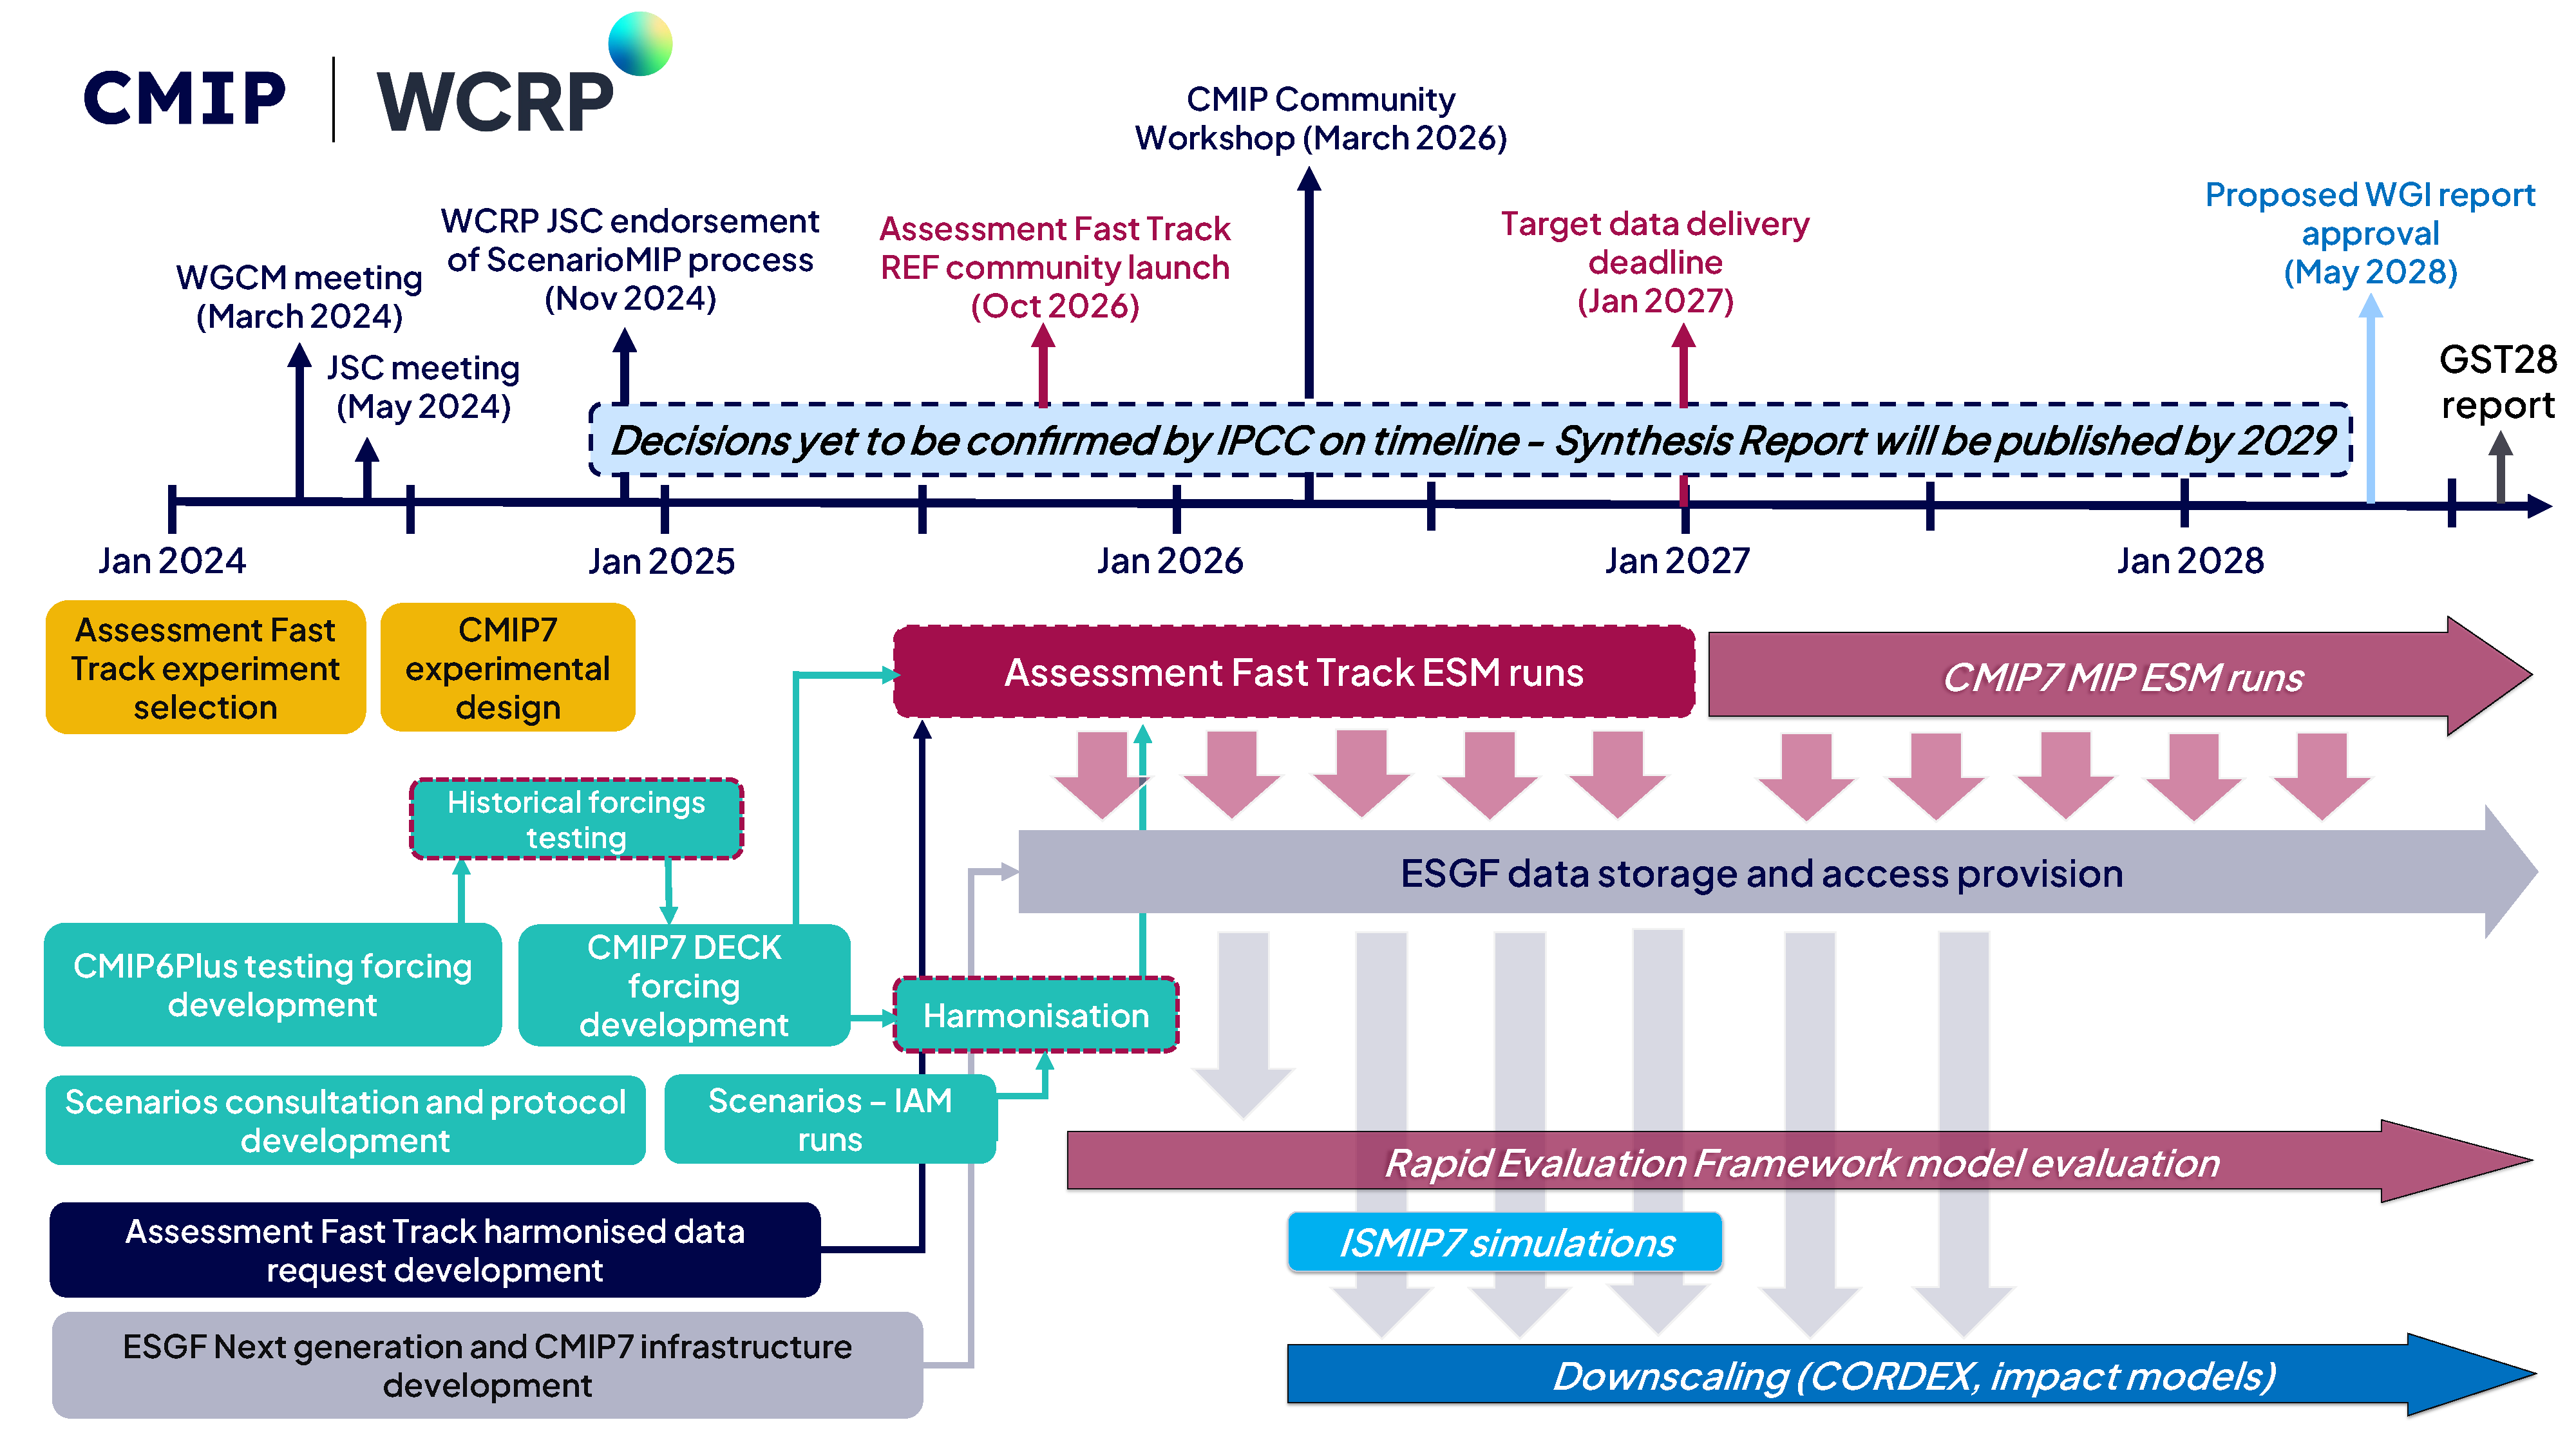
\includegraphics[width=\textwidth,angle=0]{250515_Fig1.pdf}\\
	 \caption{Timeline of the CMIP7 planning and progress - Climate forcings are essential inputs that enable modeling groups to initiate pre-industrial control and historical simulations (latest figure version is available at https://doi.org/10.5281/zenodo.15230117).}
	 \label{fig:f1}
\end{figure}


\section*{Goal 1: Latest climate-forcing dataset evaluation in preparation for CMIP7}
The first two days discussed dataset progress. Many datasets evolved from CMIP6 precedents, and new data have largely recognized and resolved identified issues during the CMIP6 and CMIP6Plus reviews. These data are now available for CMIP7 simulations to commence (Table 1).

Session one focused on latest-generation data updates. Summaries were provided for the solar, land use change, and stratospheric volcanic aerosol forcing datasets, all of which have undergone significant revisions since CMIP6. The Fresh Eyes on CMIP, a group of early career researchers, assessed early CMIP6Plus prototype datasets, providing comparisons between the preceding CMIP6- and developing data. They highlighted several issues, addressed in final data releases (Table 1). Additional discussion on forcings of the paleoclimate warm last interglacial and similar deep time periods occurred. Plans were defined to harmonize these PMIP forcings ($>$100k years earlier than present) with those covering the Holocene to present-day. All new datasets extend to 2022/2023/2024, an additional decade on the CMIP6-era data (2014 CMIP6’s last year), and offer similar spatial resolutions as preceding datasets.

In session two, discussions shifted from the recently observed past to future ScenarioMIP scenario development plans \citep{van_vuuren_scenario_2025}. First, were plans describing alignment of historical and scenario data, focused on anthropogenic emissions, associated concentrations and land use changes, along with scenario extensions past 2100. Next, the recent experience of the European RESCUE project (https://rescue-climate.eu) was described. RESCUE is one of the first projects to define scenarios including numerous carbon dioxide removal (CDR) methods for ESMs. The second last talk defined new ESM diagnostics, required to ensure accurate carbon accounting is achieved. We concluded the session with a CMIP7 ScenarioMIP plan summary, highlighting the seven illustrative scenarios, with all but one showing flat or decreasing anthropogenic GHG future emissions \citep{van_vuuren_scenario_2025}.

\subsubsection*{From Earth’s observed history to the future [potential inset box format]}
Before reviewing CMIP7 forcing status, it's important to highlight ongoing efforts to develop future scenario forcings, which run parallel to historical dataset refinement. ScenarioMIP \citep{van_vuuren_scenario_2025} defines these scenarios, initially quantified by integrated assessment models (IAMs). IAM outputs are then passed to forcing teams, who harmonize the data—ensuring smooth transitions from historical to future periods—and generate the forcings used by ESMs. These standardized datasets enable experiments spanning Earth’s past (1850–2021) to potential futures (2022–2125) and are expected to be released in July 2025 (Figure 1).

\section*{Goal 1: Latest climate-forcing dataset evaluation in preparation for CMIP7 (continued)}
The second day shifted gears. Session three focused on CMIP7 ``Diagnostic, Evaluation and Characterization of Klima'' (DECK; i.e. core experiments) protocol development. We heard from NOAA-GFDL, NCAR, and CSIRO modelers, who reported test simulation feedback with prototype CMIP6Plus datasets, along with CMIP6 data differences, and identification of issues that have been subsequently resolved. The consensus was new data reproduced the same results as previous CMIP6 data; however, more information was available in new data, such as enhanced variability quantification, and more comprehensive event coverage, particularly over the well-sampled satellite period.

Targeted talks addressed updates to volcanic, solar, and biomass-burning datasets in the context of forcing implementation for the piControl and future scenario experiments. For volcanic forcing, the uneven eruption timing complicates defining a representative pre-industrial climatology and incorporating volcanoes in future scenarios. While the satellite era is well constrained, the new dataset integrates additional ice core and geological records, expanding coverage but also increasing uncertainties in event magnitude and location. Solar forcing, active in models for decades, has seen total solar irradiance (TSI) estimates vary by $\sim$0.5\% since AMIP began in 1989 \citep{durack_coupled_2025}. The latest dataset has been enhanced to support high-top atmospheric models that simulate the mesosphere and lower thermosphere, particularly relevant for ozone modeling. An update to biomass-burning emissions was also presented, noting a step change in Northern Hemisphere variability in 1997 in the CMIP6-era dataset that induced anomalous warming across three ESMs \cite[e.g.,][]{fasullo_overview_2024,holland_new_2024}. These talks underscored the need for continued dataset refinement and better uncertainty quantification in future experiments.

A virtual forcings drop-in session was held next, providing forcing provider and CMIP modeling team engagement and discussion. Many issues were covered, with the most widely discussed being the provision of pre-industrial control (piControl) forcings. These are the key first step for modeling centers to spin-up, finalize development and freeze their CMIP7 model configurations.

In session four, we covered past forcing issues, uncertainties, a case study on implementing forcing data in ESMs, and missing datasets in the CMIP7 DECK protocol \citep{dunne_evolving_2024}. We reviewed how forcing data and model development have progressed together, with growing model complexity driving increased demands on forcing data detail and volume. The CMIP6 example of late changes to sulfate emissions in China highlighted the need for a responsive and adaptable approach, informing CMIP7’s more consultative delivery strategy. We also saw research comparing forcing datasets across two CMIP6 modeling groups, showing that changes in forcings can impact climate outcomes as much as model version differences \citep{fyfe_significant_2021,holland_new_2024}. The session underscored the central role of forcings in ESM development and the many open questions in this field.

From the modeling team perspective, IPSL described how CMIP6-era forcings were implemented to construct their simulation suite. Significant customization was needed to reformat data for model use, and updates to earlier forcings required retuning to align with observations \citep{lurton_implementation_2020}. The talk emphasized the ongoing need for clearer documentation of how ESM teams prepare and apply forcings, as even small implementation choices can lead to notably different climate outcomes. It also highlighted further opportunity for data evolution, with the potential to identify common reformatting procedures and implement this in the data development steps. 

The session then shifted to forcing datasets currently missing but needed to support evolving or absent process representations in models. First was the simple plumes parameterization—used since CMIP6 to account for aerosol radiative effects in models lacking explicit aerosol transformation schemes \citep[e.g.,][]{stevens_macv2-sp_2017,fiedler_anthropogenic_2019}. Next, the increasing freshwater input from glaciers and ice sheets was discussed. Often missing in models without interactive ice sheets, this forcing significantly influences Southern Ocean responses and is a known gap in current protocols \citep[e.g.,][]{roach_winds_2023,schmidt_anomalous_2023}. Groundwater irrigation was also highlighted—irrigated land has nearly tripled since 1950, affecting near-surface climate via soil moisture changes. Biomass burning emissions followed, with concerns about outdated pre-industrial estimates and the omission of climate-driven fire regime changes in future scenarios \citep[e.g.,][]{chen_multi-decadal_2023,hamilton_global_2024}. These omissions could introduce radiative forcing uncertainties of ~1–2 W/m² from the pre-industrial era to today \citep{hamilton_reassessment_2018,wan_importance_2021}.

The final session addressed several unmet modeling needs. These included human population and development density for estimating interactive fire ignitions; the omission of hydrogen’s global warming potential from current scenarios \citep[e.g.,][]{sand_multi-model_2023}; and the underestimation of aeolian dust, highlighted by comparison with recent reconstructions \citep[e.g.,][]{kok_mineral_2023}.

By the conclusion of the first two days, it was clear substantial work is still needed to improve confidence in climate forcings. A key challenge is bridging the sparse pre-satellite record with the better-sampled modern era to create a consistent historical timeline. New CMIP7 datasets reveal significant shifts across data stream transitions, especially for volcanic aerosols and biomass burning, emphasizing historical uncertainties. Another issue is determining the vertical injection height for anthropogenic emissions, which remains difficult even in the satellite era. Emerging research suggests that uncertainty in emission injection height has a large impact on model results, potentially affecting aerosol climate impact estimates \citep[e.g.,][]{ahsan_emissions_2023}.

In parallel, as models grow more complex, their forcing requirements increase. Many CMIP7 models in development plan to run in emissions mode—using point-source emissions instead of well-mixed concentrations—further raising the demand for detailed forcing data. Meeting these evolving needs will require continued efforts to better quantify uncertainties and improve the consistency of historical estimates.

\section*{Goal 2: From next-generation evolution to sustained revolution}
For the last two days, the meeting shifted to its second goal: the future of forcings. The aim was to recognize and document the limited support for current activities, to identify new key opportunities for future forcing development in a sustained mode and funding, and to revisit the reach and use of these datasets across an expanding user base.

Session six opened with a review of current data contributors, their observational data streams, and the support structures behind them. Over 20 funding sources across many countries were identified, including national agencies, consortia, commissions, and individual institutions supported by grants and philanthropy. Opportunities for improvement included better sharing of tools, knowledge and leveraging existing CMIP infrastructure.

The session then moved into plenaries and active discussion. The first plenary outlined downstream users—both within the World Climate Research Program (WCRP) and more broadly across the World Meteorological Organization (WMO)—and their varied weather, seasonal prediction and climate needs. Brief presentations followed, showcasing the diversity of user requirements and parallel efforts to generate forcing data for recent and regional contexts. CMIP’s long historical coverage (to 1850) was described as the ``gold standard,'' while for the well-observed modern satellite era, many alternative datasets are in use. Talks also emphasized the growing demand for higher-resolution forcings across applications like CORDEX downscaling, ECMWF seasonal forecasts, decadal predictions, Copernicus, and DestinE – with the new insight, that many of these season-decadal forecast and reanalysis activities are already leveraging the existing CMIP forcing data. Related global efforts such as the Global Carbon Project \citep{friedlingstein_global_2024} and Indicators of Global Climate Change \citep{forster_indicators_2024} were also discussed.

A key idea emerged from the discussions: while continued scientific exploration of forcings is vital, many users also need routinely produced, stable datasets. This led to the concept of updates and extensions. Updates involve revising entire datasets, including past data, to reflect new knowledge—supporting scientific progress. Extensions add only recent data without altering earlier values—critical for operational users like weather prediction centers. Balancing these needs will require new approaches, as few current workflows or funding opportunities support both effectively.

Plenary two focused on the challenges of establishing more routine forcing production, beginning with an overview of the CMIP Forcings Task Team and its funding model. An open panel followed, featuring representatives from key international agencies—including ESA, ECMWF, NOAA, the U.S. DoE, and the European Commission. Panelists expressed strong support for continued development of climate forcing datasets to meet growing demands. However, they also noted that legislative mandates and agency coordination requirements often constrain how funding can be allocated, limiting flexibility to support all user needs.

Plenaries three and four transitioned into breakout sessions, where participants explored user needs, current working models, and funding status to help define a path toward sustained forcing data delivery. The final plenary summarized key takeaways and outlined next steps, emphasizing the importance of publishing these insights to initiate broader coordination, supporting long-term and sustained Earth system forcing efforts.

\section*{Status and community next steps}
Preparations for the Coupled Model Intercomparison Project Phase 7 (CMIP7) are progressing, with a major milestone now achieved—the delivery of updated ``forcing'' datasets. These datasets are critical Earth System Model (ESM) inputs, guiding climate simulations in response to historical natural and anthropogenic changes. The ``Pathway to Regular and Sustained Delivery of Climate Forcing Datasets'' workshop brought a broad community together to advance CMIP7’s objectives. It also laid the groundwork for long-term planning, aiming to establish a sustainable framework for the ongoing provision of forcing datasets to support CMIP7, follow-on activities and a wide range of weather and climate science applications.

The meeting produced two key outcomes. First, it refined CMIP7 plans, reviewed prototype data, and outlined the delivery of forcing datasets while identifying areas for improvement and future development. More importantly, it recognized that these datasets have grown beyond their original role of standardizing model inputs, becoming foundational across Earth system science, with impact and use significantly broader than their CMIP project origins. As their use broadens across disciplines and timescales, expectations of data producers are shifting—underscoring the need to evolve collaboration models and funding structures. A central theme emerged: forcing datasets must keep pace with scientific demands to ensure robust, consistent climate and weather information. Such evolution will unlock new opportunities and strengthen the foundation for advancing Earth system science.

The workshop identified key actions to maintain CMIP7 momentum, including the need to clarify funding support for existing forcing providers, map dataset interdependencies, and assess funding agency engagement considering global political dynamics. These tasks will be shared by the CMIP Forcings Task Team and the workshop committee over the coming year, supporting both CMIP7 delivery and long-term Earth System Science planning.


\clearpage
%%%%%%%%%%%%%%%%%%%%%%%%%%%%%%%%%%%%%%%%%%%%%%%%%%%%%%%%%%%%%%%%%%%%%
% ACKNOWLEDGMENTS
%%%%%%%%%%%%%%%%%%%%%%%%%%%%%%%%%%%%%%%%%%%%%%%%%%%%%%%%%%%%%%%%%%%%%
\acknowledgments
The authors would like to thank all members of the CMIP Forcing Task Team for their tireless efforts making CMIP7 forcing datasets a reality, the European Centre for Medium-Range Weather Forecasts (ECMWF) Copernicus Climate Change Service (C3S) and the European Space Agency (ESA) for jointly hosting and sponsoring the workshop. We recognize the CMIP International Project Office (CMIP-IPO) staff, hosted by ESA, with staff provided on contract by HE Space Operations Ltd, for the exceptional workshop organization and execution. We recognize numerous international agencies supporting forcing data development. The work of P.J.D. from Lawrence Livermore National Laboratory (LLNL) is supported by the Regional and Global Model Analysis (RGMA) program area under the Earth and Environmental System Modeling (EESM) program within the Earth and Environmental Systems Sciences Division (EESSD) of the United States Department of Energy’s (DoE) Office of Science (OSTI). This work was performed under the auspices of the US DoE by LLNL under contract DE-AC52-07NA27344. LLNL IM Release: LLNL-JRNL-2002809. ZN acknowledges financial support by the CMIP International Project Office (CMIP IPO), which is hosted by the European Space Agency (ESA), the European Space Agency (ESA) as part of the GHG Forcing For CMIP project of the Climate Change Initiative (CCI) (ESA Contract No. 4000146681/24/I-LR-cl) and the European Union's Horizon 2020 research and innovation programmes (grant agreement no. 101003536) (ESM2025). HH is supported by the Met Office Hadley Centre Climate Programme funded by Department for Science, Innovation and Technology (DSIT), UK.


%%%%%%%%%%%%%%%%%%%%%%%%%%%%%%%%%%%%%%%%%%%%%%%%%%%%%%%%%%%%%%%%%%%%%
% DATA AVAILABILITY STATEMENT
%%%%%%%%%%%%%%%%%%%%%%%%%%%%%%%%%%%%%%%%%%%%%%%%%%%%%%%%%%%%%%%%%%%%%
% 
%
\datastatement
No data was generated in the production of this Meeting Report. Presented materials referred to in this document can be accessed from the workshop website at https://wcrp-cmip.org/event/forcings-workshop/.


%%%%%%%%%%%%%%%%%%%%%%%%%%%%%%%%%%%%%%%%%%%%%%%%%%%%%%%%%%%%%%%%%%%%%
% REFERENCES
%%%%%%%%%%%%%%%%%%%%%%%%%%%%%%%%%%%%%%%%%%%%%%%%%%%%%%%%%%%%%%%%%%%%%
% Make your BibTeX bibliography by using these commands:
\bibliographystyle{ametsocV6}
\bibliography{250515c}


\end{document}